\chapter{De l'insuffisance de la valorisation des données en connaissance}\label{chap:chapiter1}
\chaptermark{De l'insuffsance de la valorisation des données en connaissance}

%\minitoc

À l'ère numérique, les données se sont érigées en tant que véritable or noir de notre société, touchant presque tous les secteurs d'activité. Cependant, leur exploitation reste encore très en deçà de leur potentiel, particulièrement en ce qui concerne leur transformation en connaissances utiles et actionnables. La \autoref{sec:data_inexploitée} se penchera sur cette sous-exploitation, en examinant la situation actuelle de l'utilisation des données (\ref{subsec:current_state}), en identifiant les principales barrières à leur utilisation optimale (\ref{subsec:barrieres}), ainsi que les défis inhérents au partage de ces précieuses informations (\ref{subsec:barrieres}). Une attention particulière sera portée sur le secteur agricole, illustrant l'importance et les spécificités de l'usage des données dans ce domaine (\ref{subsec:data_in_agri}).

Face à ces défis de valorisation et de partage des données, des acteurs innovants émergent pour apporter des solutions adaptées. OKP4 SAS se distingue en tant que pionnier dans la création d'écosystèmes de données collaboratifs, visant à faciliter l'accès, la gestion, et la collaboration autour des données. Dans la section \autoref{sec:okp4_sas}, l'origine d'OKP4 SAS sera examinée (\ref{subsec:geneis_okp4}), ainsi que ses missions et sa vision pour l'avenir (\ref{subsec:missions_okp4}). De plus, les produits offerts par cette entreprise seront présentés, soulignant leur rôle essentiel dans la transformation du paysage actuel des données (\ref{subsec:produits_okp4}).

\section{La donnée : une ressource sous-exploitée} \label{sec:data_inexploitée}

\subsection{Situation actuelle de l'usage de la donnée}\label{subsec:current_state}


Dans l'ère du numérique, la quantité de données générées est faramineuse. Selon le rapport Domo de 2020, chaque minute, l'humanité produit 2,5 quintillions d'octets de données (\cite{domo_data_2020}). Pourtant, il est étonnant de constater que la grande majorité de ces données reste inexploitée. En effet, selon une estimation de l'IDC, seulement 32\% des données disponibles sont analysées et utilisées pour générer de la connaissance (\cite{reinsel_digitization_2018}).
Le coût de cette sous-exploitation est important. Selon une étude McKinsey Global Institute, si les États-Unis exploitaient pleinement le potentiel des données à grande échelle, cela pourrait augmenter le PIB du pays de 1,5\% ou 225 milliards de dollars (\cite{james_manyika_big_2011}). Cependant, malgré le potentiel économique significatif, de nombreux obstacles freinent l'exploitation efficace des données et leur valorisation en "connaissances".


\subsection{Les barrières à l'usage de la donnée}\label{subsec:barrieres}

% Selon le rapport IBM, en 2020, il y avait une demande pour près de 3 millions de spécialistes des données aux États-Unis, mais seulement une fraction de ces postes ont été pourvus \cite{ib}.
Tout d'abord, il y a un manque de compétences en matière de traitement des données. De plus, la complexité des données, souvent non structurées et volumineuses, représente un défi supplémentaire pour les organisations qui cherchent à les exploiter.

Ensuite, il y a des défis juridiques et éthiques. Les questions de confidentialité des données, de protection des données et de respect de la réglementation sont des obstacles majeurs à l'exploitation des données. Le RGPD, mis en œuvre par l'Union européenne en 2018, a accru la sensibilisation à ces questions, mais a également rendu plus difficile pour les entreprises l'exploitation des données \footnote{Le règlement général sur la protection des données (RGPD, ou encore GDPR, de l'anglais "General Data Protection Regulation"), est un règlement de l'Union européenne qui constitue le texte de référence en matière de protection des données à caractère personnel1. Il renforce et unifie la protection des données pour les individus au sein de l'Union européenne.}.

De plus, la fragmentation des données pose un problème. Les entreprises et les gouvernements ont souvent des silos de données isolés qui empêchent une analyse complète. Selon une étude de NewVantage Partners, 97\% des dirigeants interrogés affirment que leur organisation avait des difficultés à obtenir une vue d'ensemble des données en raison de cette fragmentation (\cite{noauthor_big_2020}).

Enfin, on peut citer l'insuffisance du partage de données comme un frein à l'exploitation du plein potentiel des données produites. Même si les entreprises ne manquent pas de volonté en ce sens, leurs efforts sont entravées par des barrières techniques, économiques, de sécurité et de souveraineté sur leurs données. Plus en détail, les freins au partage de données seront analysés dans la prochaine section.


\subsection{Les freins au partage de données} \label{subsec:freins_paratage}


Le partage des données est un enjeu crucial dans l'ère de l'information, offrant de nombreux avantages potentiels en termes d'innovation, de productivité et de prise de décision éclairée. Cependant, plusieurs obstacles entravent la pratique du partage des données à l'échelle mondiale.

Premièrement, les préoccupations relatives à la sécurité et à la confidentialité des données sont l'une des principales barrières au partage des données citées par les entreprises. Dans un contexte où les violations de données peuvent coûter en moyenne 4,45 millions de dollars selon le rapport de l'IBM sur le coût d'une violation de données de 2023, le manque de confiance et la réticence à partager les données est compréhensible (\cite{ibm_cost_2023}).

Deuxièmement, le manque de normes communes pour l'échange de données constitue un obstacle majeur. Sans normes communes, le transfert et l'intégration de données entre différentes entités peuvent être à la fois difficiles et coûteux.

Troisièmement, la question de la propriété des données entrave également le partage des données. En effet, la détermination de qui possède les données et qui peut en bénéficier est complexe, et souvent sujette à litige. Selon une étude du Capgemini Research Institute de 2019, 40\% des organisations estiment que les questions de propriété des données constituent un obstacle important au partage des données (\cite{capgemini_research_institute_data-powered_2019}).

Enfin, la question économique et l'alignement des intérêts divergents est aussi un gros obstacle au partage. En effet, il n'est pas rare de voir des concurrents s'engager dans cette démarche, partageant leurs données pour en obtenir de nouvelles en retour, ou encore cherchant à collaborer en échange d'une contrepartie financière, dans le cadre d'un modèle économique spécifique. Le manque de mécanismes transparents pour la valorisation des données dans ces modèles économiques constitue un frein au partage. 

%Enfin, le manque de compétences techniques peut également entraver le partage des données. Une enquête de 2021 menée par Gartner a révélé que 87\% des entreprises ont des compétences en matière de données et d'analyse inférieures à celles requises pour une exploitation efficace des données (5).

Pour surmonter ces obstacles, il est nécessaire de développer des cadres de gouvernance des données robustes, de standardiser les formats de données, d'éclaircir les questions de propriété des données et d'améliorer les compétences en matière de données et d'analyse. En surmontant ces freins, le plein potentiel des données peut être débloqué, ouvrant la voie à une nouvelle ère d'innovation et de progrès.


\subsection{L'usage de la donnée en agriculture}\label{subsec:data_in_agri}


Le secteur agricole ne reste pas en marge de ce constat d'autant plus qu'il est réputé être un secteur lent à adopter les nouvelles technologies numériques. Le McKinsey Global Institute estime que l'agriculture pourrait générer jusqu'à 1 000 milliards de dollars de valeur économique par an si les données étaient pleinement exploitées (\cite{james_manyika_digital_2016}). De plus, l'utilisation des TIC et des données pour une gestion optimisée des ressources en agriculture, pourrait réduire les coûts de production et augmenter les rendements dans le secteur qui fait partie des plus sensibles au changement climatique. Selon le Groupe d'experts Intergouvernemental sur l'Evolution du Climat (GIEC), pour chaque degré de réchauffement global, les rendements de maïs, de riz et de blé diminuent de 3 à 7\% (\cite{ipcc_global_2022}).

Toutefois, l'utilisation de la donnée pour produire des connaissances reste marginale en agriculture. Les raisons de  la sous-utilisation des données dans le secteur agricole ne s'écartent pas tellement des raisons évoquées précédemment, à savoir le manque de compétences, l'accès difficile à des données pertinentes et à des coûts adaptés, les questions juridiques de propriété intellectuelle, les questions de confidentialité et des écosystème de partage.


\section{L'apport essentiel d'OKP4 dans la structuration d'écosystèmes de données collaboratifs}
\label{sec:okp4_sas}


\subsection{Naissance de OKP4 SAS} \label{subsec:geneis_okp4}
Avant l'initiative OKP4, Emmanuel Aldeguer, président et co-fondateur de OKP4 SAS, dans ses missions de responsable Data Driven Marketing, analysait les données comptables des CUMA. Ces données pouvaient contenir des informations comme la date d'acquisition d'un tracteur qui permet de déduire sa date d'amortissement prévue, information précieuse pour un distributeur de tracteurs au moment où l'agriculteur envisage de renouveler son matériel. Grâce à OKP4, au lieu de favoriser un marché de données opaque entre comptables et vendeurs, l'idée était d'inclure l'agriculteur dans une dynamique transparente de partage de données, menée sur une plateforme commune et assortie d'une compensation.
Cette volonté a donné naissance à la raison d'être de OKP4 : transformer les données en connaissances utiles au sein d'un environnement décentralisé, transparent, ouvert et basé sur la confiance. L'objectif était d'implémenter une technologie qui faciliterait le partage sécurisé et transparent des données, respectant les consentements tout en valorisant les données.


\subsection{Missions \& Vision} \label{subsec:missions_okp4}


L'ambiton de créer OKP4 SAS a été jumelée à une prémonition : les technologies blockchain, en établissant des règles transparentes et inaltérables, pourraient servir à rémunérer les contributeurs au sein d'économies dédiées à chaque écosystème de partage de données. La vision dépeinte était celle d'une organisation décentralisée autonome, soutenue par une fondation pour assurer la pérennité du protocole.

Le projet a, dès le départ, adopté les valeurs de l'open-source, visant à construire et partager des modules technologiques qui favoriseront la création de connaissances et de valeur pour tous les acteurs des écosystèmes de partage de données. Les outils, comme les langages, les frameworks et les bibliothèques, sont exempts de droits de propriété intellectuelle, permettant la réutilisation et l'amélioration du code par d'autres projets.

Prochainement, une entreprise, du nom de Pollen, est envisagée pour fournir des services autour du protocole OKP4 et contribuer à sa maintenance. Cela comprend la création d'espaces de données, la prestation de plateformes de données en tant que service, le développement du protocole OKP4 et la gestion d'actifs numériques. Cette entreprise, serait un acteur clé pour favoriser et soutenir la pérennité du protocole OKP4. Par ailleurs, une association va naître dans les prochains mois en Suisse pour animer la communauté autour du protocole, coordonner son développement par des prestataires comme Pollen ainsi que par sa communauté de developpeur open-source.

\begin{figure}
    \centering
    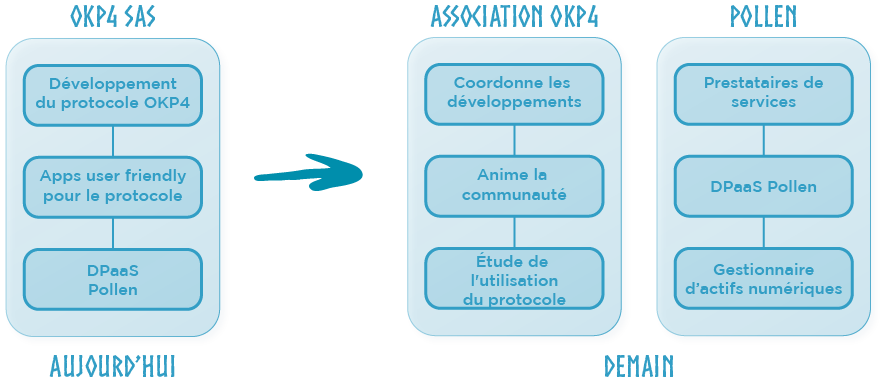
\includegraphics[width=0.8\textwidth]{ILLUSTRATIONS/okp4_td_dm_bis_update.png}
    \caption{OKP4 aujourd'hui vs demain}
    \label{fig:okp4_today_tomorrow}
\end{figure}


\subsection{Produits et services de OKP4 SAS} \label{subsec:produits_okp4}


OKP4 propose une gamme étendue de services et de produits innovants qui exploitent pleinement le potentiel de l'écosystème décentralisé de partage de données qu'elle a contribué à créer.

\begin{itemize}
\item \textbf{Développement du protocole OKP4}

     Ce protocole open-source constitue le cœur technologique de l'écosystème. Il a été conçu pour favoriser le partage de données sécurisé, transparent et respectueux du consentement des utilisateurs. L'équipe d'OKP4 est activement impliquée dans son développement continu, aidé par la communauté open source, travaillant sans relâche pour l'optimiser et l'adapter aux évolutions des besoins des utilisateurs et des avancées technologiques.
     
    \item \textbf{Développement d'applications}
    
    OKP4 est engagée dans la création d'applications utilisateur qui facilitent l'interaction avec le \textit{dataverse} \footnote{dataverse}. Ces applications sont conçues pour être intuitives et faciles à utiliser, tout en offrant une myriade de fonctionnalités pour explorer, exploiter et gérer les données au sein de l'écosystème de partage.
    \item \textbf{Offre de Data Platform as a Service (DPaaS) : Pollen}

    Pollen est l'offre de Data Plateform en tant que service de OKP4 SAS qui offre aux entreprises et organisations un accès facile et flexible aux ressources du \textit{dataverse}. Avec cette plateforme, les clients peuvent bénéficier de la puissance et de la flexibilité du partage de données décentralisé sans avoir à gérer les difficultés d'utilisation du Web3 \footnote{Le Web3 ou Web 3.0 est un terme utilisé pour désigner l'idée d'un web décentralisé exploitant la technologie des chaînes de blocs (blockchain), se voulant ainsi le successeur du Web 2.0, terme utilisé pour désigner le web "social" .}. 

    Pollen s'intègre en effet au-dessus de \textit{data spaces} sur mesure - des écosystèmes de partage de données. Ces \textit{data spaces} évolutifs dans leurs gouvernances, permettent aux entreprises de s'engager en toute confiance dans l'économie de la connaissance sans perte de souveraineté sur leurs données. Dans le cadre de l'offre Pollen, OKP4 se charge de la création et de la maintenance de ces espaces, permettant ainsi aux clients de se concentrer sur l'exploitation des données pour générer des connaissances et créer de la valeur.
    

    \item \textbf{Application de Business Intelligence en marque blanche}

En complément de ses services, OKP4 SAS a également développé une application dédiée à la Business Intelligence. Cet outil permet aux clients d'analyser et d'interpréter les indicateurs créés, leur offrant ainsi une meilleure compréhension de leurs opérations et une base solide pour la prise de décision. En facilitant l'accès à des insights précieux, cette application de Business Intelligence contribue à maximiser l'exploitation des données et à créer de la valeur pour les utilisateurs.

\end{itemize}

\newpage
